\vspace{-1cm}
\begin{wrapfigure}[16]{r}{7cm}
  \centering
  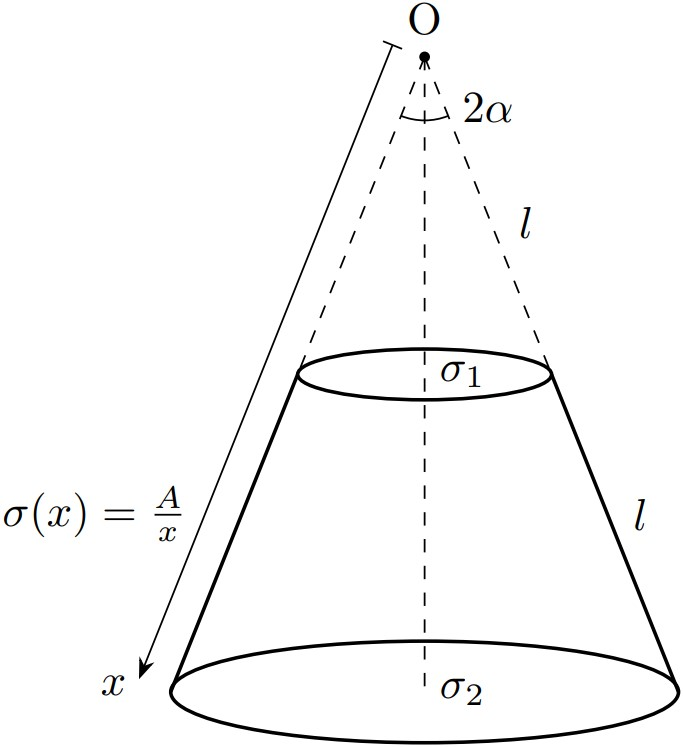
\includegraphics[width=0.38\textwidth]{Figures/Fig 3.jpg}
  \begin{center}
    \figurename{ 3}
  \end{center}
\end{wrapfigure}

\noindent Một khối đặc có dạng nón cụt, không dẫn điện, được tích điện trên mặt bên sao cho mật độ điện tích mặt thay đổi theo khoảng cách $x$ đến đỉnh $O$ theo công thức $\sigma(x)=A/x$ với $A$ là một hằng số dương đã biết. Đáy trên và đáy dưới của hình nón cụt được tích điện đều với mật độ điện tích tương ứng là $\sigma_{1}$ và $\sigma_{2}$. Độ dài đường sinh và nửa góc ở đỉnh của hình nón đầy đủ lần lượt là $2l$ và $\alpha=30^{\circ}$, độ dài đường sinh của hình nón cụt là $l$.
\begin{enumerate}
  \item Giả sử $\sigma_{1}=-\sigma_{2}=\sigma_{0}$ với $\sigma_{0}$ là một giá trị đã biết. Xác định độ lớn điện trường $E_{O}$ tại điểm $O$ trên hình 3.
\end{enumerate}
Bên trong hình nón cụt, người ta đục một lỗ nhỏ dọc theo trục đối xứng của nó. Một điện tích thử $-q$ với $q>0$, khối lượng $m$, có thể di chuyển không ma sát bên trong lỗ này. Giả sử $\sigma_{1}=\sigma_{2}=\sigma_{0}$.
\begin{enumerate}
  \setcounter{enumi}{1}
  \item Xác định khoảng cách từ vị trí cân bằng của điện tích thử bên trong hình nón cụt tới điểm $O$. Đồng thời, hãy chỉ ra rằng, khoảng cách này không phụ thuộc vào $\sigma_{0}$.
  \item Với giá trị nào của $\sigma_{0}$ thì cân bằng của điện tích thử ở vị trí vừa tìm được ở ý trên là bền? Tìm chu kỳ dao động bé của điện tích thử quanh vị trí cân bằng này.
\end{enumerate}
Trong suốt bài toán, hình nón cụt được giữ cố định. Cho biết hằng số điện môi của vật liệu làm nên hình nón cụt là $\varepsilon=1$, bỏ qua tác dụng của trọng lực và các hiện tượng từ tính.\\